
\begin{figure*}[ht]
    \centering
    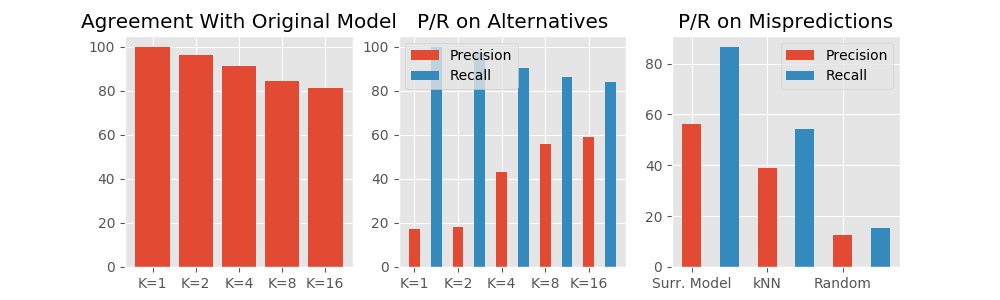
\includegraphics[width=\textwidth]{figures/result1.png}
    \caption{(A) Illustrates how well a debuggable surrogate model can approximate a complex model, (B) illustrates how well this surrogate model can isolate mispredictions in terms of precision and recall, and (C) why alternative approaches do not work.}
    \label{fig:teaser}
\end{figure*}

\section{Highlighted Results}
We present an illustrative example in this paper to describe its applications to supervised learning.
We have a dataset of movie descriptions IMDB~\footnote{ \url{ftp://ftp.fu-berlin.de/pub/misc/movies/database/}} and Yahoo~\footnote{ \url{http://webscope.sandbox.yahoo.com/catalog.php?datatype=r}}.
Each movie has a title, a short 1-2 paragraph plot description, year, rating, language, and a list of categories, and the goal is to train a model to predict whether a movie is a ``Horror'' or ``Comedy'' from the description and title.  
The total dataset has 506,244 records.

First, using TensorFlow, we trained a LSTM-based model to predict these categories. The first layer of this model computes what is called a word-embedding, where the LSTM learns a feature-space in which similar words (co-occuring) are closer together. 
The next two layers consist of dense layers that map the words from the feature-space to classification outputs.
The result is a model that achieves 93\% accuracy, which is far more accurate than simpler alternatives on a Bag-of-Words featurization (random forests 90\%, Linear SVM 81\%, Kernel SVM 85\%).
The problem is that it is hard to diagnose what this model is exactly doing, unlike the simpler alternatives. 

We applied our approach to learn a surrogate model that approximates the original one (Figure \ref{fig:teaser}). We varied the number of submodels $k$ to illustrate the tradeoff. Figure \ref{fig:teaser}a shows the agreement between the surrogate and the original model as a function of $k$. As the model is increasingly compartmentalized with a higher $k$ the agreement goes down, however, not too drastically. The next plot shows how well the surrogate model can isolate related records (Figure \ref{fig:teaser}b). We randomly sample 10 mispredictions of the model, and identify the submodel that mispredicted those examples. We then query all of the data that contributed to that submodel and measure how effective that submodel is at extracting other mispredictions (in terms of precision and recall).
As $k$ increases, we see an increased ability to isolate errors, but the surrogate increasingly deviates from the original model.
Finally, we compare the algorithm to baselines to show that it is far more accurate than random guessing or a simple k-Nearest Neighbor search in TFIDF space (Figure \ref{fig:teaser}c).


